\definecolor{lineColor}{RGB}{50,50,50}
\definecolor{boxBg}{RGB}{250,250,250}
\definecolor{accentBlue}{RGB}{0,114,178}
\definecolor{accentRed}{RGB}{213,94,0}

% Heatmap colors (Muted professional scale)
\definecolor{h1}{RGB}{232,242,250}
\definecolor{h2}{RGB}{187,215,233}
\definecolor{h3}{RGB}{124,176,209}
\definecolor{h4}{RGB}{62,137,185}
\definecolor{h5}{RGB}{5,99,155}

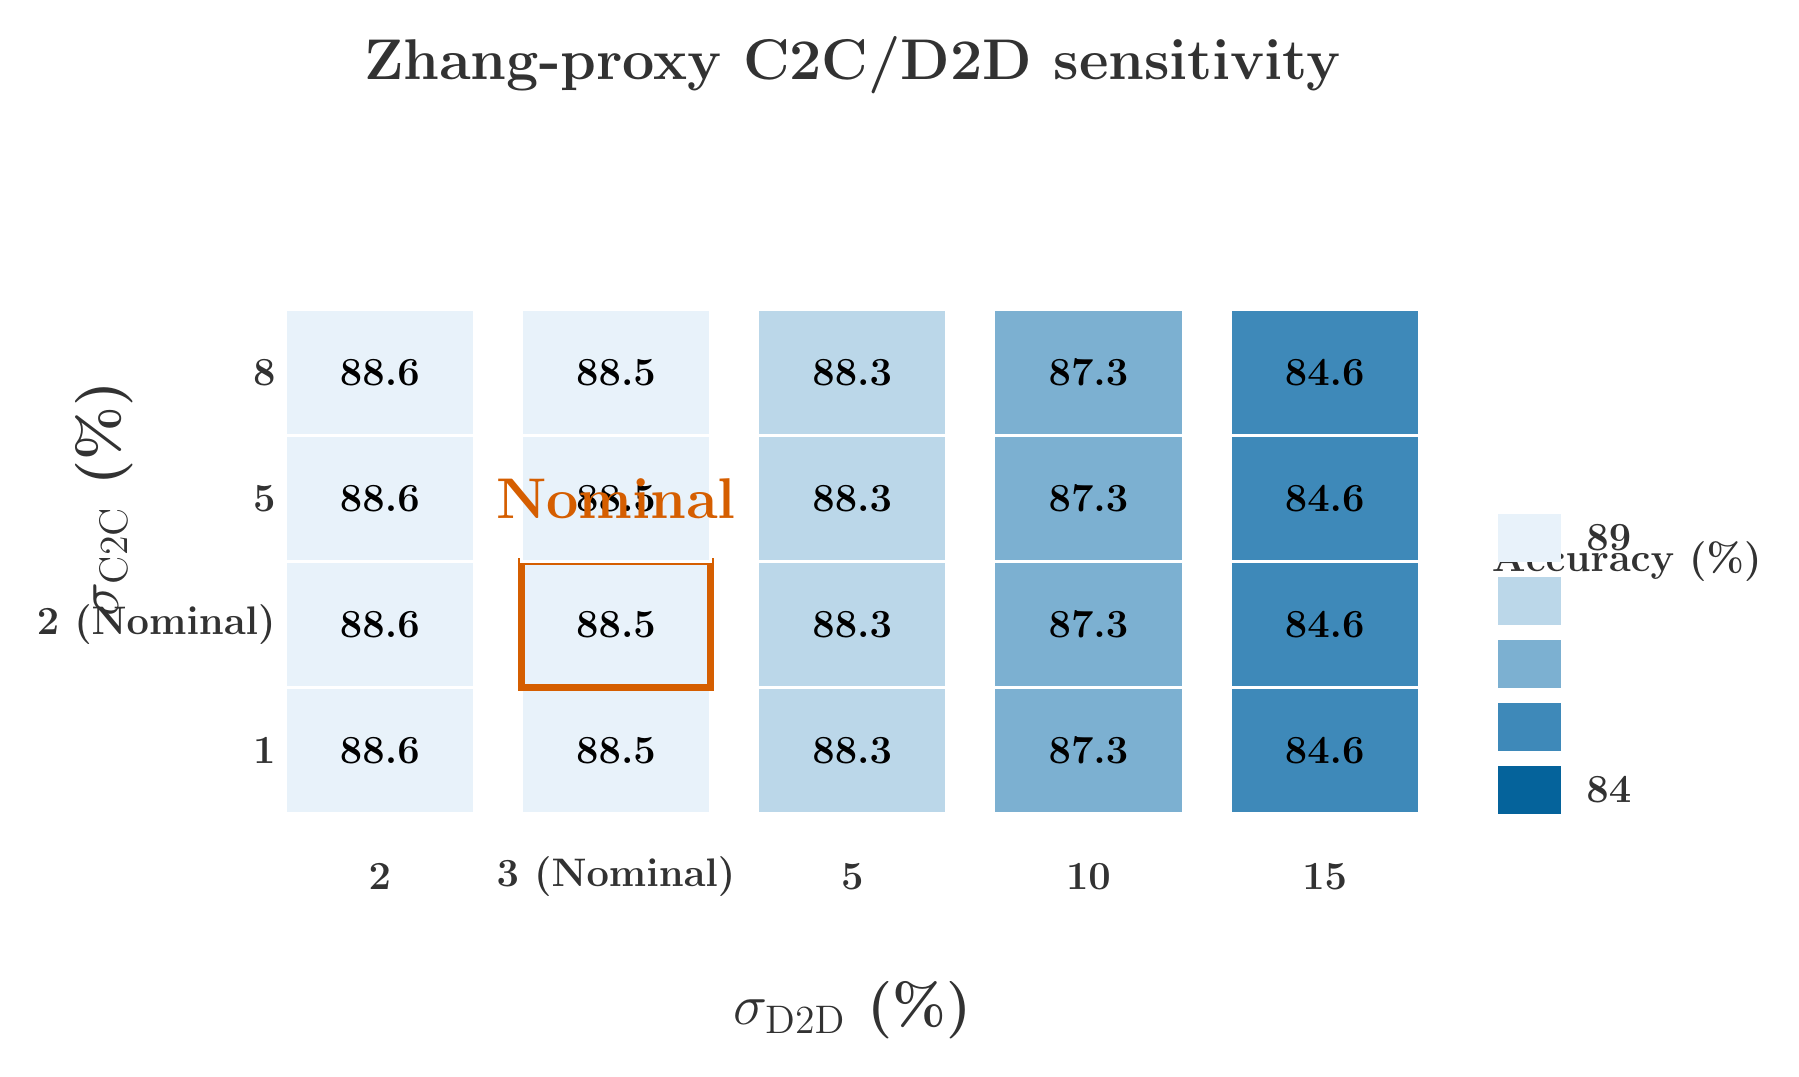
\begin{tikzpicture}[
  scale=1.0, transform shape,
  font=\sffamily,
  cell/.style={draw=white, line width=1.0pt, minimum width=2.4cm, minimum height=1.6cm, align=center, font=\Large\bfseries},
  label/.style={font=\Large\bfseries, text=lineColor},
  title/.style={font=\huge\bfseries, text=lineColor},
  axislabel/.style={font=\huge\bfseries, text=lineColor}
]

% Centered Title
\node[title] at (6.0, 9.5) {Zhang-proxy C2C/D2D sensitivity};

% Y-axis label
\node[axislabel, rotate=90] at (-3.5, 4.0) {$\sigma_{\mathrm{C2C}}$ (\%)};

% X-axis label
\node[axislabel] at (6.0, -2.5) {$\sigma_{\mathrm{D2D}}$ (\%)};

% X-axis ticks
\node[label] at (0, -0.8) {2};
\node[label] at (3, -0.8) {3 (Nominal)};
\node[label] at (6, -0.8) {5};
\node[label] at (9, -0.8) {10};
\node[label] at (12, -0.8) {15};

% Y-axis ticks
\node[label, anchor=east] at (-1.2, 0.8) {1};
\node[label, anchor=east] at (-1.2, 2.4) {2 (Nominal)};
\node[label, anchor=east] at (-1.2, 4.0) {5};
\node[label, anchor=east] at (-1.2, 5.6) {8};

% Data grid (C2C rows bottom to top, D2D cols left to right)
% D2D: 2 (h1), 3 (h1), 5 (h2), 10 (h3), 15 (h4)

% C2C = 1%
\node[cell, fill=h1] at (0, 0.8) {88.6};
\node[cell, fill=h1] at (3, 0.8) {88.5};
\node[cell, fill=h2] at (6, 0.8) {88.3};
\node[cell, fill=h3] at (9, 0.8) {87.3};
\node[cell, fill=h4] at (12, 0.8) {84.6};

% C2C = 2%
\node[cell, fill=h1] at (0, 2.4) {88.6};
\node[cell, fill=h1, draw=accentRed, line width=2.5pt] at (3, 2.4) {88.5}; % Nominal point
\node[cell, fill=h2] at (6, 2.4) {88.3};
\node[cell, fill=h3] at (9, 2.4) {87.3};
\node[cell, fill=h4] at (12, 2.4) {84.6};

% C2C = 5%
\node[cell, fill=h1] at (0, 4.0) {88.6};
\node[cell, fill=h1] at (3, 4.0) {88.5};
\node[cell, fill=h2] at (6, 4.0) {88.3};
\node[cell, fill=h3] at (9, 4.0) {87.3};
\node[cell, fill=h4] at (12, 4.0) {84.6};

% C2C = 8%
\node[cell, fill=h1] at (0, 5.6) {88.6};
\node[cell, fill=h1] at (3, 5.6) {88.5};
\node[cell, fill=h2] at (6, 5.6) {88.3};
\node[cell, fill=h3] at (9, 5.6) {87.3};
\node[cell, fill=h4] at (12, 5.6) {84.6};

% Legend
\node[anchor=west, label] at (14.0, 3.2) {Accuracy (\%)};
\foreach \i/\c in {0/h5, 1/h4, 2/h3, 3/h2, 4/h1} {
    \fill[\c] (14.2, 0.0 + \i*0.8) rectangle (15.0, 0.6 + \i*0.8);
}
\node[label, anchor=west] at (15.2, 0.3) {84};
\node[label, anchor=west] at (15.2, 3.5) {89};

% "Nominal" marker label
\node[accentRed, font=\huge\bfseries] at (3, 4.0) {Nominal};

\end{tikzpicture}
